\newcommand{\mycomb}{% two rays 
    \draw[->] (0,0)-- (6*\dx,0) node[right] {};

    \foreach \i in {1,...,5}{
        \draw[->] ({\i*\dx},0) -- ({\i*\dx},\dy) node[above]{};
    }
}

\begin{figure}[ht]
\centering
\begin{tikzpicture}
    \def\radius{0.15}
    \def\dy{3}
    \def\dx{1.5}

    \mycomb

    \only<2->{
    \foreach \i in {2,...,5}{
    \begin{scope}[shift = {({\i*\dx},0)},rotate = 90,scale = 0.33]
        \mycomb
    \end{scope}
    }
    }

    \only<3->{
    \foreach \i in {3,...,5}{
    \foreach \j in {1,...,5}{
    \begin{scope}[shift = {({\i*\dx},0)},rotate = 90,scale = 0.33]
        \begin{scope}[shift = {({\j*\dx},0)},rotate = 90,scale = 0.33]
            \mycomb
        \end{scope}
    \end{scope}
    }
    }
    }
\end{tikzpicture}
\end{figure}